\section{Zielsetzung}
\label{sec:Zielsetzung}

In diesem Versuch soll die Herauslösung von Elektronen aus Metallen (hier: Wolfram)
mithilfe des glühelektrischen Effekts untersucht werden. Von besonderem Interesse
ist hier die Temperaturabhängigkeit dieses Effekts.

\section{Theorie}
\label{sec:Theorie}

\subsection{Leitungselektronen in Metallen}

Metalle haben eine Gitterstruktur und eine sehr gute 
elektrische Leitfähigkeit, welche durch die auf dem 
Kristallgitter sitzenden ionisierten Atome zu begründen
ist.
Die Ionen sind durch diese Gitterstruktur räumlich
periodisch verteilt und werden von freigesetzte Elektronen
eingehüllt, welche keinem bestimmten Atom mehr zuzuordnen
sind. Sie befinden sich stattdessen im Kraftfeld sämtlicher
Atome in dem Kristallgitter.
Diese Elektronen werden \textit{Leitungselektronen} genannt.
Die Ionen stellen durch die Abwesenheit der Elektronen
eine positive Ladungsquelle dar. Daher nimmt das Gitterpotential
in der Nähe dieser Gitterpunkte hohe positive Werte an.
Weiter entfernt ist das Potential allerdings näherungsweise
konstant.

Mit dieser Näherung kann das Metallinnere als ein Gebiet
angesehen werden, in dem ein konstantes positives Potential
herrscht. Dieses Potential ist um den Betrag $\xi$
vom Außenraum verschieden. Damit Elektronen das Metall
verlassen können, müssen diese also eine Potentialbarriere
der Höhe $\xi$ überwinden. Dargestellt ist dies 
in \autoref{Abb:Potentialtopf}.\\

\begin{figure}[H]
    \centering  
    \caption{Potentialtopf-Modell eines Metalls.\cite{sample}}
    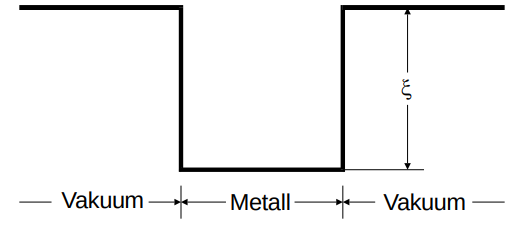
\includegraphics[width=\textwidth]{Bilder/Potentialtopf.png}
    \label{Abb:Potentialtopf}
\end{figure}

\subsection{Austrittsarbeit der Elektronen}

Um gegen dieses Potential anlaufen zu können, muss eine
\textit{Austrittsarbeit} $\mathrm{e}_0 \xi$ geleistet
werden. Die Konstante $\mathrm{e}_0$ ist hier die
Elementarladung.
Es stellt sich nun die Frage, ob die Elektronen dieses
Potential ohne zusätzliche Energie Zufuhr verlassen können.
Also ob die innere Energie der Elektronen hoch genug ist.
Die Quantentheorie liefert hier eine zufriedenstellende 
Antwort:\\
Aus der Quantentheorie wissen wir, dass Elektronen 
nur bestimmte Energiewerte $E_{\mathrm{n}}$ annehmen können.
Für Teilchen mit halbzahligen Spin gilt das Pauli-Verbot.
Jedes solches Teilchen muss sich in einem anderen Quantenzustand
befinden. Elektronen sind solche Teilchen. Für jedes Energieniveau
gibt es nur eine endliche Zahl an möglichen Quantenzahlen,
daher ḿuss das Energieniveau immer weiter steigen.
Dies führt dazu, dass selbst beim absoluten Nullpunkt
Elektronen noch eine endliche Energie besitzen, welche im 
Mittel $\frac{3}{2} k_{\mathrm{B}} T$ ist. Die Maximalenergie
ist abhängig von der Anzahl der Elektronen pro Volumeneinheit 
im Metall. Diese Maximalenergie ist die Fermische Grenzenergie
$\zeta$. Bei Zimmertemperatur gilt $\zeta \, >> \, kT$. Die
Wahrscheinlichkeit ein Elektron bestimmter Energie bei 
bestimmter Temperatur (beim thermischen Gleichgewicht) berechnet
sich zu 
\begin{equation}
    \label{eqn:FermiDirac}
    f(E) = \frac{1}{\exp{\left(\frac{E - \zeta}{k_{\mathrm{B}}T}\right)}+1}.
\end{equation}
Diese Gleichung ist die \textit{Fermi-Diracsche Verteilungs-Funktion}.
$E$ ist die Energie des Teilchens, $\zeta$ die Maximalenergie,
$T$ die Temperatur und $k_{\mathrm{B}}$ die Boltzman-Konstante.
Der Verlauf dieser Kurve ist in \autoref{Abb:FermiDirac} dargestellt.

\begin{figure}[H]
    \centering
    \caption{Graphischer Verlauf der \textit{Fermi-Diracsche Verteilungs-Funktion} bei T = 0 K und T >> 0 K.\cite{sample}}
    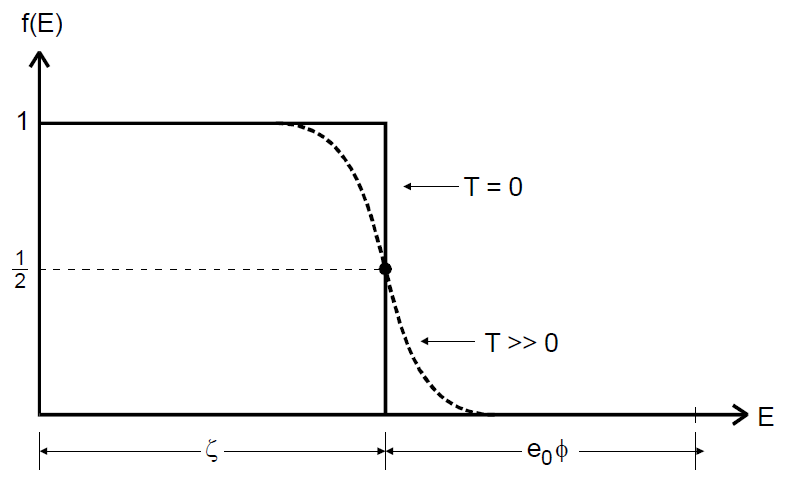
\includegraphics[width=\textwidth]{Bilder/FermiDirac.png}
    \label{Abb:FermiDirac}
\end{figure}

Anhand der Graphik ist gut zu sehen, dass ein Elektron die Energie $\zeta + e_0 \xi$
besitzen muss, damit es die Metalloberfläche verlassen kann. Selbst bei Temperaturen
ähnlich dem Schmelzpunkt von jenen Metallen (hier: Wolfram) ist dieser Energiewert
immer noch groß gegenüber $kT$, sodass die Exponentialfunktion bei \autoref{eqn:FermiDirac}
>> 1 ist. Für Elektronen mit hoher Energie kann man also die
Annäherung 
\begin{equation}
    \label{eqn:FermiDiracKurz}
    f(E) \approx \exp{\left(\frac{\zeta - E}{kT}\right)}
\end{equation}
verwenden.

\subsection{Sättigungsstromdichte bei der thermischen Elektronenemission}

Mit der vereinfachten Version der \textit{Fermi-Diracsche Verteilungs-Funktion} 
(\autoref{eqn:FermiDiracKurz}) lässt sich sie Sättigungsstromdichte $j_S(T)$ herleiten.
Die Sättigungsstromdichte gibt an, wie viele Elektronen pro Zeit- und Flächeneinheit 
aus der Metalloberfläche austreten. Diese Stromdichte ist temperaturabhängig. Die Zahl
$\mathrm{d}\alpha$  der Elektronen, die auf die Oberfläche treffen beträgt $\mathrm{d}\alpha=v_z \, n(E) \, \mathrm{d}p_x \,
\mathrm{d}p_y \, \mathrm{d}p_z$. Mit der kinetischen Energie $ E = \frac{1}{2 m_0} \left(p_x^2 + p_y^2 +p_z^2\right) = 
\frac{m_0}{2}\left(v_x^2 + v_y^2 + v_z^2\right)$ lässt sich die die Anzahl der Elektronen
zu 
\begin{equation*}
    \mathrm{d}\alpha = n(E) \mathrm{d}E \, \mathrm{d}p_x \, \mathrm{d}p_y
\end{equation*}
berechnen. Im sechsdimensionalen Phasenraum nimmt jeder Quantenzustand das Volumen $h^3$ 
ein, daher ergibt sich $n(E) = \frac{2}{h^3} f(E)$ und unser Ausdruck für die 
Elektronenanzahl erweitert sich zu 
\begin{equation*}
    \mathrm{d}\alpha = \frac{2}{h^3} \exp{\left(\frac{\zeta - E}{kT}\right)} \mathrm{d}E \, \mathrm{d}p_x \, \mathrm{d}p_y.
\end{equation*}
Die Stromdichte $j_S(T)$ erhält man nun indem man alle Elektronen, deren Energiekomponente senkrecht zur Metalloberfläche die Ungleichung
$ \frac{p_z^2}{2m_0} > \zeta + e_0 \xi$ erfüllen summiert und mit der Elementarladung multipliziert.
Nach trivialen Umformungen ergibt sich für die Sättigungsstromdichte der Ausdruck
\begin{equation}
    \label{eqn:Saettigung}
    j_S(T) = 4\pi \frac{e_0 m_0 k^2}{h^3} T^2 \exp{\left(\frac{-e_0 \xi}{kT}\right)}
\end{equation}
\autoref{eqn:Saettigung} ist auch unter \textit{Richardson-Gleichung} bekannt.

\subsection{Langmuir-Schottkysche Raumladungsgleichung}
Bei Verwendung des in \autoref{sec:Versuchsaufbau} gezeigten Versuchsaufbaus stellt man 
fest, dass der Anodenstrom von der Kathodentemperatur und Anodenspannung abhängig ist. Wenn
die Spannung nicht hoch genug ist, erreichen nicht mehr alle Elektronen
die Auffanganode. Wenn die Spannung allerdings hoch genug ist, erhält man einen von der
Anodenspannung unabhängigen Strom. Hier ist das Ohmsche Gesetz also nicht mehr gültig.
Das ist jedoch auch bereits vor dieser hohen Spannung der Fall, da die Geschwindigkeit der
Elektronen nicht konstant ist. Diese werden zur Anode hin beschleunigt, wodurch die 
Raumladungsdichte $\rho$ der Elektronen eine Funktion des Ortes innerhalb der Diode ist. Die 
Raumladungsdichte der Elektronen beeinflusst den Verlauf der Feldstärke zwischen Anode und Kathode.
Es folgt, dass die von der Anode ausgehenden Feldlinien nicht mehr alle bis zur Kathode reichen,
sondern bereits an den Raumladungselektronen enden. Die emittierten Elektronen werden
folglich nicht mehr alle vom Anodenfeld erfasst. Der Diodenstrom der gemessen wird ist also
kleiner als der zu erwartende Sättigungsstrom. Mit diesen Erkenntnissen folgt nach einigen
Umformungen der Zusammenhang zwischen Stromdichte $j$ und Anodenspannung $V$:
\begin{equation}
    \label{eqn:Langmuir}
    j = \frac{4}{9} \epsilon_0 \sqrt{2 \frac{e_0}{m_0}} \frac{V^{3/2}}{a^2}
\end{equation}
Diese Gleichung heißt das \textit{Langmuir-Schottkysche Raumladungsgesetz}.

\subsection{Anlaufstromgebiet einer Hochvakuumdiode}

Aus der \autoref{eqn:Langmuir} würde logisch folgen, dass für keine Anodenspannung auch
die Stromdichte verschwindet. Im Experiment lässt sich allerdings beobachten, dass trotzdem
ein geringer Anodenstrom fließt. Das liegt daran, dass die Elektronen die Kathode mit einer gewissen 
Geschwindigkeit verlassen. Die kinetische Energie ist der Energieüberschuss, die die Elektronen
nach dem Verlassen aus dem Material haben. Diese ergibt sich zu
\begin{equation}
    \symup{\Delta} E = E - (\zeta + e_0 \xi).
\end{equation}
Der nun gemessene Anodenstrom ist der \textit{Anlaufstrom}. Die Potentialverhältnisse
in einer Hochvakuumdiode im Bereich ihres Anlaufstromgebiets ist in \autoref{Abb:Anlauf}
dargestellt.

\begin{figure}[H]
    \centering
    \caption{Potentialverhältnisse in einer Hochvakuumdiode im Bereich ihres \textit{Anlaufstromgebietes}.\cite{sample}}
    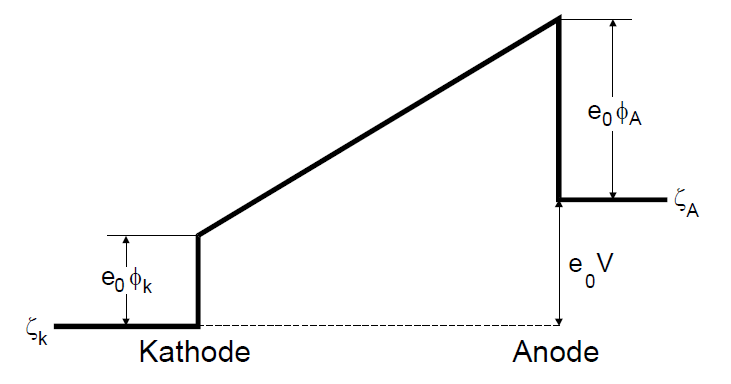
\includegraphics[width=\textwidth]{Bilder/Anlauf.png}
    \label{Abb:Anlauf}
\end{figure}

Es ist zu erkennen, dass diejenigen Elektronen die die Anode erreichen eine Energie 
von $e_0 \xi_A + e_0 V$ haben müssen. $e_0 \xi_A$ ist die benötigte Austrittsarbeit der
Anode. $V$ ist ein äußeres Potential. Es ergibt sich folgende Abhängigkeit der Anlaufstromstärke
vom äußeren Potential $V$:
\begin{equation}
    \label{eqn:AnlaufStrom}
    j (V) = j_0 \exp{\left(-\frac{e_0 \xi_A + e_0 V}{kT}\right)}
\end{equation}

\subsection{Kennlinien der Hochvakuumdiode}

Die Kennlinie einer Hochvakuumdiode ist der Zusammenhang zwischen Stromdichte und
Anodenstrom. In den verschiedenen Raumgebieten der Anoden sieht dieser Zusammenhang 
unterschiedlich aus. Insgesamt kann der Raum in Anlaufstromgebiet, Raumladungsgebiet
und Sättigungsstromgebiet aufgeteilt werden. Die drei Kennlinien sind in 
\autoref{Abb:Kennlinien} dargestellt.
\begin{figure}[H]
    \centering
    \caption{\textit{Kennlinien} einer Hochvakuumdiode.\cite{sample}}
    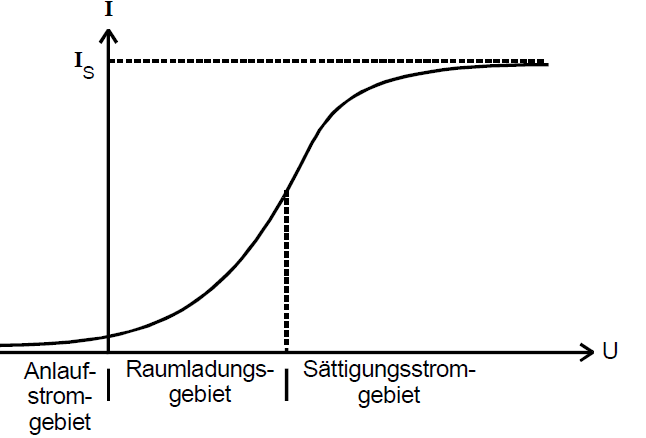
\includegraphics[width=\textwidth]{Bilder/Kennlinien.png}
    \label{Abb:Kennlinien}
\end{figure}